\documentclass{report}
\usepackage{setspace} % Setting line spacing
\usepackage{ulem} % Underline
\usepackage{caption} % Captioning figures
\usepackage{subcaption} % Subfigures
\usepackage{geometry} % Page layout
\usepackage{multicol} % Columned pages
\usepackage{array,etoolbox}
\usepackage{fancyhdr}
\usepackage{enumitem}
\usepackage{amsmath}
\usepackage[toc,page]{appendix}
\setlist{noitemsep}

% Page layout (margins, size, line spacing)
\geometry{letterpaper, left=1in, right=1in, bottom=1in, top=1in}
\setstretch{1}

% Headers
\pagestyle{fancy}
\lhead{PeaPod - Solution Overview}
\rhead{UpRoute Development Foundation}

\begin{document}

\begin{titlepage}
    \begin{center}
        \vspace*{1.2cm}

        \textbf{\large{PeaPod - Solution Overview}}

        \vspace{0.5cm}

        Outlining a Design Proposal to the Deep Space Food Challenge

        \vfill \small{

            \textbf{Jayden Lefebvre - Lead Engineer, Founder of UpRoute Development Foundation}\\
            BASc Computer Engineering (Anticipated 2024), University of Toronto\\
            Toronto, ON, Canada\\
            \vspace{.5cm}
            \textbf{Nathan Chareunsouk - Design Lead}\\Toronto, ON, Canada\\
            \vspace{.5cm}
            \textbf{Navin Vanderwert - Design Engineer}\\
            BASc Engineering Science (Anticipated 2024), University of Toronto\\
            Toronto, ON, Canada\\
            \vspace{.5cm}
            \textbf{Jonas Marshall - Electronics Engineer}\\
            BASc Computer Engineering (Anticipated 2024), Queen's University\\
            Kingston, ON, Canada

        }

        \vspace{1cm}

        Primary Contact Email: jayden.lefebvre@mail.utoronto.ca

        \vspace{.75cm}

        Revision 0.9\\
        UpRoute Development Foundation\\
        Aug 4th, 2021

    \end{center}
\end{titlepage}

\thispagestyle{plain}

\tableofcontents
\newpage

\section{Introduction}
\label{sec:intro}

\subsection{Purpose \& Design Process}
\label{sec:purpose}

The purpose of this document is to outline a design proposed to meet the PeaPod Requirements. It accomplishes this via the following process:

\begin{figure}[h]
    \centering
    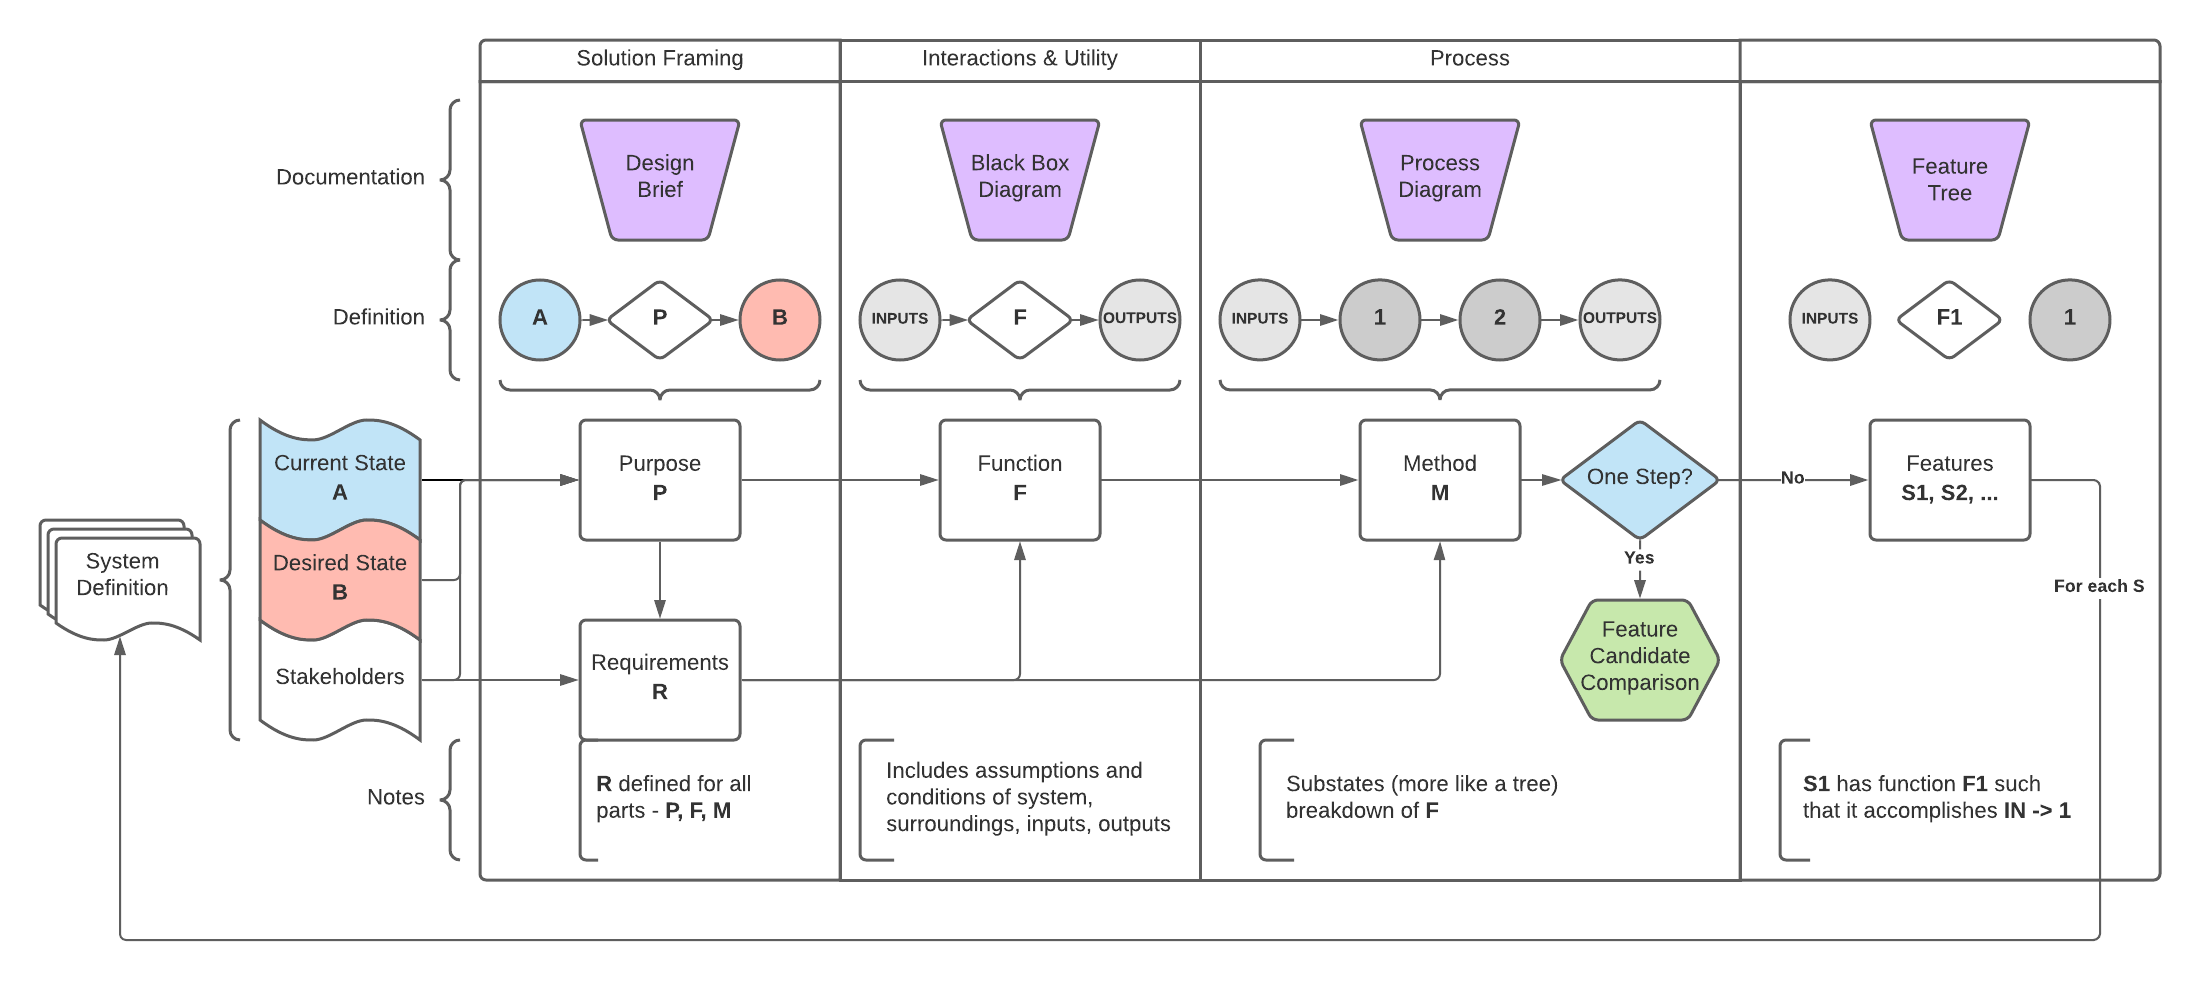
\includegraphics[height=7.55cm,angle=90,origin=c]{images/designprocess.png}
    \hfill
    \caption{Engineering design process.}
\end{figure}

\newpage

\section{Design}

\textbf{Purpose}: An automated and isolated aeroponic crop growth system, able to generate any growth environment from a combination of independent environment parameters, with both environment and crop growth data collection for optimization.

\textbf{Function}:
\begin{itemize}
    \item \textbf{Infrastructural Inputs}: Water, nutrient solutions, pH solutions, power, network connection, plant seeds/clones
    \item \textbf{Information Inputs}: Plant identifiers, environment program, input solution identifiers
    \item \textbf{Products}: Edible plant matter, recorded environment data, plant metric data, timelapse
    \item \textbf{Byproducts}: Inedible plant matter, heat from thermoregulation cooling
\end{itemize}

\textbf{Method}:
\begin{enumerate}
    \item \textit{Setup}:
    \begin{enumerate}
        \item Assemble housing, trays;
        \item Install control module(s) (CM);
        \item Hook up all inputs, fill solution containers;
        \item For each tray, either:
        \begin{enumerate}
            \item Mount lighting boards and driver, daisy chain boards to driver, hook up power and signal to driver and CM; \textbf{OR}
            \item Mount aeroponic nozzle mount and arm, hook up water delivery line to nozzles and CM;
        \end{enumerate}
        \item Prepare and plant seeds for desired crop output, seal growth environment;
        \item Setup all other systems;
    \end{enumerate}
    \item \textit{Process}:
    \begin{itemize}
        \item Aeroponics system supplies plants with necessary water and nutrients at set pH;
        \item Lighting systems meet all photosynthetic, etc. light requirements;
        \item Environment control systems record and maintain desired environment conditions:
        \begin{itemize}
            \item Air temperature;
            \item Air humidity;
            \item Root zone temperature;
            \item Air composition;
        \end{itemize}
    \end{itemize}
    \item \textit{Shutdown}:
    \begin{enumerate}
        \item \textbf{End-of-Program}: Harvest, storage, and (eventual) preparation and consumption of edible plant matter (now food products);
        \item \textbf{End-of-Life}: Inedible plant matter is scrapped. New plants may be planted.
    \end{enumerate}
\end{enumerate}

\textbf{Features}:
\begin{itemize}
    \item \textit{Housing}: Section \ref{sec:housing}.
    \item \textit{Automation}: Sensing and actuating all systems autonomously. Section \ref{sec:automation}. Systems include:
    \begin{itemize}
        \item \textit{Aeroponics}: Section \ref{sec:aeroponics}.
        \item \textit{Environmental Control}: Section \ref{sec:environment}.
        \item \textit{Lighting}: Section \ref{sec:lighting}.
    \end{itemize}
\end{itemize}

\newpage

\subsection{Automation}
\label{sec:automation}

\textbf{Purpose}: Performing growth-, maintenance-, and data-related tasks autonomously on the basis of both schedule and necessity to reduce crew maintenance time. Maintains the homogeneity of the internal environment. Increased accuracy/precision over human interference, minimize human hours spent. Enables control over all parameters simultaneously.

\textbf{Function}:
\begin{itemize}
    \item \textbf{Inputs}: Environment sensor reading signals, program
    \item \textbf{Outputs}: Actuator control signals, crew messaging
\end{itemize}

\textbf{Method}:
\begin{enumerate}
    \item \textit{Setup}:
    \begin{enumerate}
        \item Power is connected and system is booted;
        \item Program is inputted by user;
    \end{enumerate}
    \item \textit{Testing}:
    \begin{itemize}
        \item Power-on Self-Test (POST) passes;
        \item Systems enact program as intended;
    \end{itemize}
    \item \textit{Process}:
    \begin{enumerate}
        \item Checks operating preconditions (self POST and per-subsystem);
        \item \textbf{Environment Control Loop} (matches \textit{Sense-Plan-Act} model of robotics):
        \begin{enumerate}
            \item Receives and stores data about current environment state;
            \item Compares current state to desired state, develops a "plan" to reach desired state;
            \item Controls subsystem operations in order to enact the plan;
        \end{enumerate}
        \item Notifies user on maintenance requirement (i.e. non-automated input/output management, refills, repairs, etc.) and end-of-program (EOP);
    \end{enumerate}
    \item \textit{Shutdown} (either manual or EOP):
    \begin{enumerate}
        \item Stop subsystem operations;
    \end{enumerate}
\end{enumerate}

\textbf{Features}:
\begin{itemize}
    \item \textit{Computer System}: Manages \textbf{all} data collection, storage, analysis, and transmission/receiving, as well as planning and actuator control. Includes internal clock (for program, notification), network connection (for data transmission, notification), and storage (for data). 
    \item \textit{Camera \& Plant Metrics}: Multiple angles. For live feed transmission to users (local and remote), as well as plant health and yield metric collection via \textbf{computer vision analysis}. Matches $\vec P$ from the optimization routine (\ref{sec:optimization}). Metrics include:
    \begin{itemize}
        \item Leaf health indicators (i.e. leaf tip burn, leaf curl, chlorosis);
        \item Leaf count, size distribution;
        \item Leaf density;
        \item Canopy dimensions/surface area;
        \item Plant height;
        \item Fruit/harvest body size, ripeness;
        \item etc.
    \end{itemize}
    \item \textit{Environment Sensors}: Record the environment's current state. Covers each environment control loop (see \ref{sec:environment} \textbf{outputs}). Matches $\vec E$ from the optimization routine (\ref{sec:optimization}).
\newpage
    \item \textit{Diagnostic Systems}: Include informative sensors tracking system input availability, etc. as well as notification triggers.
    \item \textit{Program}: Set of action (e.g. lights on) and control target (e.g. hold air temperature at 22°C) \textbf{time-series} instructions;
    \item \textit{Actuator Control}: Induce a change. Covers each environment control (see \ref{sec:environment}, \ref{sec:lighting} \textbf{inputs});
\end{itemize}

\vspace{1cm}

\subsection{Housing}
\label{sec:housing}

\textbf{Purpose}: \textit{Isolates} and \textit{insulates} growth environment from surroundings (heat, light, water vapour, air). Provides structural integrity and mounting points for other subsystems. Enables system extendability via repeated "unit cell" topology.

\textbf{Method}:
\begin{enumerate}
    \item \textit{Setup}:
    \begin{enumerate}
        \item Construct frame and install panels;
        \item Mount control module (w/ subsystems), connect inputs and internal subsystem connections;
        \item Install tray mounts, insert trays (w/ subsystems);
    \end{enumerate}
    \item \textit{Testing}:
    \begin{itemize}
        \item Frame construction is rigid, level, and sturdy;
        \item Panels are insulating against temperature changes;
    \end{itemize}
    \item \textit{Process}:
    \begin{enumerate}
        \item Panels insulate against heat gain/loss, are opaque, and contain light and heat via reflection;
        \item Shell construction is tight, thus sealing against moisture;
        \item Internal vertical mounting channels for systems, horizontal plane "trays";
        \item \textbf{Extension} (can be repeated):
        \begin{enumerate}
            \item Add a second housing;
            \item Remove dividing panel from both housings;
            \item Remove "shared" skeleton extrusions from second housing;
            \item Join the two housings to form one larger 2x1 housing;
            \item \textbf{Extension Modes} (may be combined in any way to suit application):
            \begin{itemize}
                \item \textit{Option 1} (Smaller Housings): Operate the combined housing off \textbf{one} control module.
                \item \textit{Option 2} (Larger Housings): Add control modules to account for additional air volume, plant count, power requirement, etc.. Operate in a \textbf{controller-follower topology}.
                \item \textit{Option 3} (Frame Connection Only): Leave the dividing panel, add a control module, and operate the two PeaPods \textbf{separately}.
            \end{itemize}
        \end{enumerate}
    \end{enumerate}
    \item \textit{Shutdown}:
    \begin{enumerate}
        \item Dismount all systems, remove trays;
        \item Disassemble housing;
    \end{enumerate}
\end{enumerate}

\newpage

\textbf{Features}:
\begin{itemize}
    \item \textit{Frame}: T-slotted aluminum extrusion framing with aluminum face-mounted brackets forms a cubic skeleton for rigidity/strength (high strength-to-weight aluminum) and easy component mounting and repositioning (standard mounting channels). These extrusions form the "edges" of the cubic housing. %Todo: cite extrusion
    \item \textit{Panels}: Graphite-enhanced expanded polystyrene (GPS) rigid foam insulation panels \cite{insulation} with reflective mylar internal lamination increase energy efficiency (GPS RSI of 0.0328$\frac{m^2 \cdot \degree C}{W}$ per mm of thickness, mylar enables light/heat reflection), as well as safety against cross-contamination and pathogens. Panels slide into extrusion channels and form a "seal" for greater water vapour retention. These panels form the "faces" of cube. %Todo: cite mylar
    \item \textit{Trays}: Horizontal plane subframes mounted to internal vertical extrusion channels for ease of repositioning. Trays slide in/out on permanent mounts. All connections are quick-connect (i.e. quick-diconnect tubing for grow tray, push connectors for lighting) for ease of removal. Trays include:
    \begin{itemize}
        \item \textit{Grow Trays}: Support plants (via grow cups), aeroponic nozzles, aeroponics container, and supply/recycling lines (See \ref{sec:aeroponics}).
        \item \textit{Lighting Trays}: Support LED boards, driver board (See \ref{sec:lighting}).
    \end{itemize}
\end{itemize}

\vspace{1cm}

\subsection{Aeroponics}
\label{sec:aeroponics}

\textbf{Purpose}: Delivers nutrients and pH-balanced, temperature-controlled water to the plant roots via a fine mist.

\textbf{Function}:
\begin{itemize}
    \item \textbf{Inputs}: Reverse osmosis water\footnote{RO water has no dissolved nutrients and a neutral pH of 7.0. This enables easier and more reliable calculations. In addition, it has no particulate or minerals, minimizing the chances of nozzle clog.} under positive pressure, pH up \& down solutions, concentrated nutrient solutions, pump control (on/off to relay for pump power), nozzle control (on/off to relay for solenoid power), pH and nutrient solution ratios as signals (stepper positions/valve open percent), thermoregulation power as signal (PWM to H-bridge polarity switch to MOSFET to Peltier), thermoregulation fan power
    \item \textbf{Outputs}: Mist (50 micron mean droplet diameter), runoff water
\end{itemize}

\textbf{Method}:
\begin{enumerate}
    \item \textit{Setup}:
    \begin{enumerate}
        \item Hook up all inputs;
        \item Connect the quick-disconnect fitting;
        \item Fill nutrient, pH solution containers;
        \item Calibrate pressure, temperature sensors to atmospheric;
        \item Enable water input to prime system (if known pressure/temperature, calibrate sensors);
        \item Mount container, connect runoff output line to extraction port;
    \end{enumerate}
\newpage
    \item \textit{Testing}:
    \begin{itemize}
        \item Temperature, pressure sensors communicate as expected;
        \item No leaks at any connections under a) source pressure, b) fully pressurized;
        \item Pump auto-shuts off near 80PSI;
        \item Tubing and all components withstand full pressurization;
        \item Solenoid is normally closed, withstands full pressurization, and opens when power is applied;
        \item Quick-disconnect operates as intended at full pressurization without leaks;
        \item Nozzles produce full-cone mist;
        \item Manual and servo-actuated valves operate as intended;
        \item Runoff container is sealed, and extraction port works;
    \end{itemize}
    \item \textit{Process}:
    \begin{enumerate}
        \item Water is pressurized to constant 80PSI;
        \item Heat is added to or removed from the water (\ref{sec:automation}); % TODO: Add water temp to environment control?
        \item Temperature and pressure of the water is read (feeds back);
        \item Nutrient and pH (\ref{sec:nutrientsph}) solutions are mixed in-line at an adjustable ratio (\ref{sec:automation}); \footnote{I.e. add X mL of nutrient solution Y per mL water to achieve Z ppm, or add A mL of pH down solution per mL water to achieve a pH of B.}
        \item Flow to nozzle is controlled (on/off) (\ref{sec:automation});
        \item Nozzle turns pressurized water into mist, which is 98\% more water efficient than traditional farming;
        \item Mist runoff is contained by a container, and extracted for processing as waste water;
    \end{enumerate}
    \item \textit{Shutdown}:
    \begin{enumerate}
        \item Extract all remaining runoff;
        \item Power down the pump and thermoregulation unit;
        \item Close the nutrient and pH solution valves;
        \item Close the source shutoff valve;
        \item Open the drain valve, and allow the system to depressurize and  drain completely;
        \item Power down the solenoid;
        \item Disconnect the quick-disconnect fitting;
        \item Disconnect the inputs;
    \end{enumerate}
\end{enumerate}

\textbf{Features} (in order of plumbing; source $\to$ nozzle):
\begin{itemize}
    \item \textit{Water Source}: Input for reverse-osmosis water.
    \item \textit{Manual Source Shutoff Valve}
    \item \textit{Diaphragm Pump}: Self-priming, auto-shutoff at 80psi. Power is controlled by external relay signal (\ref{sec:automation}).
    \item \textit{Inline Water Heater/Cooler}: Thermoelectric heater/cooler. Peltier tiles (H-bridge polarity control, PWM dimming), aluminum water block/heat sink combo, and fans.
    \item \textit{Accumulator Tank}: Uses an air bladder to create and stabilize pressure.
    \item \textit{Pressure Sensor}: Reports to computer (\ref{sec:automation}). Allows for shutoff of pump in case of emergency.
    \item \textit{Manual Drain Valve}: Ball valve. Allows the system to be depressurized and drained.
    \item \textit{Nutrient and pH Adjustment Solutions}: Section \ref{sec:nutrientsph}
    \item \textit{Adjustable-rate Siphon Injection Manifold}: Section \ref{sec:manifold}.
    \item \textit{Solenoid Valve}: Enables on-demand (\ref{sec:automation}) misting.
    \item \textit{Grow Tray Quick-Disconnect}: Connectors between aeroponics supply and nozzles that allow for quick disconnection with auto-shutoff so the trays may be removed.
    \item \textit{Nozzle}: Mounted to grow tray, pointed at plant roots. 80psi water through a 0.4-0.6mm orifice produces 5-50 micron water droplets, optimal for plant growth. %TODO: Source??
    \item \textit{Runoff Collection Container}: Mounted and \textbf{sealed} to the grow tray. Encapsulates the nozzles and root zone \textbf{entirely}, and provides a runoff water extraction port.
\end{itemize}

\vspace{.5cm}

\subsubsection{Solution Nutrients and pH}
\label{sec:nutrientsph}

\textbf{Purpose}: Providing all necessary plant nutrients at the correct pH.

\textbf{Function}:
\begin{itemize}
    \item \textbf{Inputs}: Plant nutrients, pH up solution, pH down solution (all stored)
    \item \textbf{Outputs}: Plant nutrients, pH up solution, pH down solution (on-demand)
\end{itemize}

\textbf{Method}:
\begin{enumerate}
    \item \textit{Setup}:
    \begin{enumerate}
        \item Fill containers with nutrient, pH solutions;
        \item Install and connect fill level sensors;
        \item Install output tubes;
    \end{enumerate}
    \item \textit{Testing}:
    \begin{itemize}
        \item No container leaks;
        \item Fill level sensors operate as intended;
    \end{itemize}
    \item \textit{Process}:
    \begin{enumerate}
        \item Solutions are held in containers;
        \item Solutions are siphoned from containers on-demand;
        \item Fill level sensors notify user (\ref{sec:automation}) when empty;
    \end{enumerate}
    \item \textit{Shutdown}:
    \begin{enumerate}
        \item Empty containers;
        \item Disconnect fill level sensors and output tubes;
    \end{enumerate}
\end{enumerate}

\textbf{Features}:
\begin{itemize}
    \item \textit{Nutrient Solutions}: Aqueous. Highly concentrated. Selectable as part of the program (\ref{sec:automation})\footnote{Many different solutions can be combined (according to solubility laws, pH requirements, etc.).}, and may include any of:
    \begin{itemize}
        \item Bioavailable nonmetals (ammonia, ammonium, nitrates, nitrites, phosphates, sulfates, etc.)
        \item Bioavailable metals (potassium, etc.)
        \item Minerals (magnesium, calcium)
        \item Other trace elements
        \item Custom solutions (i.e. fungicides/algicides)
    \end{itemize} 
    \item \textit{pH Adjustment Solutions}\footnote{\textit{NOTE:} Ionic composition of pH solutions should be considered in the understanding of the spray (i.e. phosphic acid results in phosphate ions in spray)}: Aqueous. Highly concentrated. One for pH up (>8), one for pH down (<6).
    \item \textit{Solution Storage Containers}: Opaque, insulated, chemical-safe, refillable cartridges. Prevent degradation of solution compounds over time via light or heat.
    \begin{itemize}
        \item \textit{Fill Level Sensors}: Depth sensors measure fill level of container. Notifies user to refill.
    \end{itemize}
\end{itemize}

\vspace{.5cm}

\subsubsection{Solution Injection Manifold}
\label{sec:manifold}

\textbf{Purpose}: A manifold of parallel in-line injectors, allowing for adjustable mixing ratios for nutrient and pH solutions.

\textbf{Function}:
\begin{itemize}
    \item \textbf{Inputs}: Pressurized RO water, per-solution flow-ratio control signal (calculated from desired per-nutrient concentrations; \ref{sec:automation}), pH flow-ratio control signal (calculated from desired pH; \ref{sec:automation})
    \item \textbf{Outputs}: Pressurized mixed solution with set pH and nutrient concentrations
\end{itemize}

\textbf{Method}:
\begin{enumerate}
    \item \textit{Setup}:
    \begin{enumerate}
        \item Connect inlet lines to siphon inlets;
        \item Connect solution containers to inlet lines;
        \item Connect flow control servos to control module;
    \end{enumerate}
    \item \textit{Testing}:
    \begin{itemize}
        \item Flow control servos and valves operate as intended;
        \item Injection ratios are accurate;
        \item Check valves prevent backflow when solenoid is closed;
    \end{itemize}
    \item \textit{Process}:
    \begin{enumerate}
        \item Water splits into parallel injection "branches";
        \item Each branch injects solution at an adjustable (\ref{sec:automation}) ratio (flow:flow);
        \item Branches recombine;
    \end{enumerate}
    \item \textit{Shutdown}:
    \begin{enumerate}
        \item Disconnect inlet lines from siphons, containers;
        \item Disconnect flow control servos from control module;
    \end{enumerate}
\end{enumerate}

\textbf{Features}:
\begin{itemize}
    \item \textit{Venturi Siphons}: Venturi-based siphons for flow-ratio injection of solutions (one siphon per solution).
    \item \textit{Input, Output Manifold}: Manifolds for distribution of water to branches, and recombination of solution post-injection.
    \item \textit{Flow Control Valves}: Completely adjustable flow control, driven by servos.
    \item \textit{Check Valves}: Prevents backflow through siphon inlet when output solenoid is closed.
\end{itemize}

\newpage

\subsection{Environment Control}
\label{sec:environment}

\textbf{Purpose}: Subsystems responsible for generating the internal plant growth environment, providing control over all relevant environment parameters. Provides sensing and acting peripherals to the control module's automation system (\ref{sec:automation}).

\textbf{Function}:
\begin{itemize}
    \item \textbf{Inputs}: Power, water, environment control parameters (as signals)
    \item \textbf{Outputs}: Environment sensor values, controlled environment
\end{itemize}

\textbf{Method} (informed by \ref{sec:automation}):
\begin{enumerate}
    \item \textit{Setup}:
    \begin{enumerate}
        \item Connect power, water inputs;
        \item Connect all actuator input signals and sensor output signals to control module;
    \end{enumerate}
    \item \textit{Testing}:
    \begin{itemize}
        \item Each subsystem responds properly to automation (\ref{sec:automation}) control;
        \item Each control loop system sensor reports accurately;
    \end{itemize}
    \item \textit{Process}:
    \begin{enumerate}
        \item Sensor signals sent to automation (\ref{sec:automation});
        \item Actuator control signals received from automation (\ref{sec:automation});
        \item Actuators respond to control signals to control:
        \begin{itemize}
            \item Leaf zone air temperature\footnotemark[4];
            \item Leaf zone humidity\footnotemark[4];
            \item Root zone/aeroponics temperature\footnote{Control Loop (aka Feedback) System - includes sensor(s)};
            \item Air Composition (CO${}_2$/O${}_2$)\footnotemark[4];
            \item Lighting spectrum and intensity\footnote{Set System - no feedback sensors};
            \item Aeroponics delivery/"flow" rate\footnotemark[5];
            \item Aeroponics solution per-nutrient concentrations\footnotemark[5];
            \item Aeroponics solution pH\footnotemark[5];
        \end{itemize}
    \end{enumerate}
    \item \textit{Shutdown}:
    \begin{enumerate}
        \item Disconnect inputs;
        \item Disconnect control module connections;
    \end{enumerate}
\end{enumerate}

\textbf{Features}:
\begin{itemize}
    \item \textit{Aeroponics System} (\ref{sec:aeroponics}), with:
    \begin{itemize}
        \item \textit{Solution Dosing} (\ref{sec:nutrientsph})
        \item \textit{Solution Heater, Cooler} (\ref{sec:watertemp})
    \end{itemize}
    \item \textit{Air Heater, Cooler} (\ref{sec:airthermoregulation})
    \item \textit{Air Humidifier} (\ref{sec:airhum}), \textit{Dehumidifier} (\ref{sec:dehum})
    \item \textit{Gas Exchanger} (\ref{sec:gas})
    \item \textit{Lighting} (\ref{sec:lighting})
\end{itemize}

\newpage

\subsubsection{Air Thermoregulation}
\label{sec:airthermoregulation}

\textbf{Purpose}: Maintaining desired leaf-zone air temperature and circulating air.

\textbf{Function}:
\begin{itemize}
    \item \textbf{Inputs}: Power, air temperature control signal (\ref{sec:automation}), air circulation control signal (\ref{sec:automation});
    \item \textbf{Outputs}: $\pm$Heat to environment, $\mp$heat to surroundings, internal air circulation, internal air temperature sensor signal (\ref{sec:automation});
\end{itemize}

\textbf{Method}:
\begin{enumerate}
    \item \textit{Testing}:
    \begin{itemize}
        \item Heat pump direction and magnitude respond to control signal as expected;
        \item Fans operate as expected;
        \item Heat pump power exceeds maximum heat loss (temperature extremes)\footnote{i.e. if X Watts leave the system at MAX°C internal, MIN°C external, the heat pump can transfer >X Watts};
        \item Heat pump power exceeds that required to reach temperature extremes in under sixty (60) seconds given the system's heat capacity;
    \end{itemize}
    \item \textit{Process}:
    \begin{enumerate}
        \item Air is circulated throughout the environment;
        \item Temperature is measured, sent to control module;
        \item Control module controls heat pump speed and direction (heating vs. cooling);
    \end{enumerate}
\end{enumerate}

\textbf{Calculations}:

Assuming an atmospheric pressure $P$ of 101.325kPa, a surroundings temperature range $T_{surr-min}$, $T_{surr-max}$ of 18-24$\degree$C, a system target temperature range $T_{sys-min}$, $T_{sys-max}$ of 13-30$\degree$C, and a single-housing arrangement (6 faces), a molar mass of dry air\footnote{Water vapour has a maximum concentration of 30g/kg at 30$\degree$C, or 3\%, which is irrelevant for mass and heat capacity calculations.} $M$ of 28.97 $\frac g{mol}$, a specific heat capacity of dry air $c_p$ of $1.006 \frac{J}{g*\text{K}}$ and a 4-unit (2x2) expanded configuration:\\
\vspace{.05cm}
\begin{gather*}
    \label{eqn:heatloss}
    Q_{loss}=\frac{(T_{surr-min}-T_{sys-max}) * A}{\text{RSI per mm} * \ell}=\frac{(22\degree \text{C}-30\degree \text{C}) * (16 \text{ faces} * 0.5\text{m} * 0.5\text{m})}{0.0328 \text{m}^2~  \degree \text{C}~\text{W}^{-1}~\text{mm}^{-1} * 20 \text{mm}}=-48.78 W\\\vspace{.05cm}\\
    \label{eqn:airmass}
    m_{air}=\frac{P*V*M}{R*T_{avg}}=\frac{101325\text{Pa}*(0.5\text{m}*0.5\text{m}*0.5\text{m}*4\text{ units})*28.97\frac g{mol}}{8.314\frac{J}{\text{mol}*K}*300\text{K}}=588.4g\\\vspace{.05cm}\\
    \label{eqn:heatcapacity}
    W_{heating}=\frac{m*c_p*(T_{surr-min}-T_{sys-max})}{t}=\frac{588.4g*1.006\frac{J}{g*\text{K}}*(22\degree \text{C}-30\degree \text{C})}{60\text{ sec}}=-78.92\text{W}
\end{gather*}

$\therefore$ An 80W thermoelectric system will supply enough power to heat/cool the box in 60 seconds AND more than enough to maintain temperature.

\newpage

\textbf{Features}:
\begin{itemize}
    \item \textit{Circulation Fans}: Located in growth environment to circulate air even temperature distribution.
    \item \textit{Temperature Sensors}: SHT31 \cite{sht31} sensors on breakout boards located throughout the growth environment to measure air temperature. Informs a \textbf{PID control loop} (\ref{sec:automation}).
    \item \textit{Heat Pump}: Pumps heat in or out of the growth environment. Is comprised of:
    \begin{itemize}
        \item \textit{Peltier Devices}: 2x50W bidirectional solid-state \textbf{thermoelectric devices} (Peltier tiles) \cite{peltier} pump heat from one face to the other. Better space efficiency, less complexity (no liquids, pressurized fluids, etc.), and more precise than other methods.
        \item \textit{Peltier Driver Circuit}: Controls direction and magnitude of Peltier device heat pump via a \textbf{MOSFET H-bridge} and \textbf{dimmable current source} respectively.
        \item \textit{Heat Sinks}: Aluminum blocks with fins hold and exchange heat between air and Peltier devices. One set on each side of the Peltier (inside and outside environment) builds "heat pump". Mating face coated with thermal compound for better transfer.
        \item \textit{Heat Sink Fans}: Located on both sets of heat sinks for better heat dissipation.
    \end{itemize}
\end{itemize}

\subsubsection{Air Humidification}
\label{sec:airhum}

\textbf{Purpose}: Actively \textit{increases} growth environment air humidity.

\textbf{Function}:
\begin{itemize}
    \item \textbf{Inputs}: Power, humidification on/off control signal (\ref{sec:automation}), RO water\footnote{RO water contains no minerals/particulate, and as such prevents the common problem of mesh clog/calcification.};
    \item \textbf{Outputs}: Water vapour, humidity sensor signal;
\end{itemize}

\textbf{Method}:
\begin{enumerate}
    \item \textit{Setup}:
    \begin{enumerate}
        \item Connect humidification control signal to control module;
        \item Connect humidity sensor signal to control module;
        \item Connect RO water line to water tank;
    \end{enumerate}
    \item \textit{Testing}:
    \begin{itemize}
        \item Humidification unit responds to control signal as expected;
        \item Humidity sensor reads as expected;
        \item Tank does not leak;
    \end{itemize}
    \item \textit{Process}:
    \begin{enumerate}
        \item Water is delivered to a small tank (nebulizer is mounted);
        \item Power and control signal activate a nebulizer driver;
        \item Nebulizer vapourizes water;
    \end{enumerate}
    \item \textit{Shutdown}:
    \begin{enumerate}
        \item Disconnect RO water line and drain tank;
        \item Disconnect humidification control signal and humidity sensor signal from control module;
    \end{enumerate}
\end{enumerate}

\textbf{Features}:
\begin{itemize}
    \item \textit{Circulation Fans}: See Section \ref{sec:airthermoregulation}.
    \item \textit{Humidity Sensor}: Located throughout the growth environment to measure air humidity. Informs a \textbf{bang-bang} control loop (\ref{sec:automation});
    \item \textit{Humidification Unit}: Easily controllable and produces a consistent vapour. Comprised of:
    \begin{itemize}
        \item \textit{Water Tank}: Holds a small amount of water behind the piezoelectric mesh.
        \item \textit{Piezoelectric Mesh Disc}: Oscillates in such a way that vapour is generated when water is passed over it. Mounted to the water tank.
        \item \textit{Driver Circuit}: Fixed-frequency\footnote{113kHz for 20mm disc} 555 timer circuit driving an amplifier/LC circuit generates an AC signal. Powers the piezoelectric disc.
    \end{itemize}
\end{itemize}

\newpage

\subsubsection{Air Dehumidification}
\label{sec:dehum}

\textbf{Purpose}: Actively \textit{decreases} growth environment air humidity.

\textbf{Function}:
\begin{itemize}
    \item \textbf{Inputs}: Humid air (high water vapour content), dehumidification control signal (shutter servo open/close, fan speed), dry desiccant
    \item \textbf{Outputs}: Dry air (low water vapour content), saturated desiccant
\end{itemize}

\textbf{Method}:
\begin{enumerate}
    \item \textit{Setup}:
    \begin{enumerate}
        \item Dehumidification control signals are hooked up;
        \item Dry desiccant is added to cartridge, which is inserted;
    \end{enumerate}
    \item \textit{Testing}:
    \begin{itemize}
        \item Desiccant removes moisture from air;
        \item Desiccant indicates saturation as expected, which is sensed by computer;
        \item Shutters operate as intended, and no dehumidification occurs when closed;
        \item Maximum dehumidification rate exceeds total plant transpiration rate;
    \end{itemize}
    \item \textit{Process}:
    \begin{enumerate}
        \item Humidity sensor sends data to control module (\ref{sec:automation});
        \item Dehumidification control signal activates fans and opens shutters;
        \item Humid air passes over the desiccant, and dry air exits the unit;
        \item Desiccant becomes saturated, and indicates this;
        \item Indication is sensed by computer (\ref{sec:automation}), which notifies the user;
        \item Cartridge is removed by the user, and swapped for a dry one. Process continues;
        \item Saturated cartridge is recharged;
    \end{enumerate}
    \item \textit{Shutdown}:
    \begin{enumerate}
        \item Control signals are disconnected;
        \item Final recharging of cartridge;
        \item Desiccant is removed from cartridge;
    \end{enumerate}
\end{enumerate}

\textbf{Calculations}:

Assuming an air temperature of 30$\degree$ C, water vapour saturation of $30.4g/m^{3}$, RH of 90\%, target RH of 20\%, and 6\% weight dessicant capacity:
\vspace{.05cm}
\begin{gather*}
    90\% RH = 0.90 * 30.4g/m^{3} = 27.36g/m^{3} \\
    20\% RH = 0.20 * 30.4g/m^{3} = 6.08g/m^{3} \\
    Vol_{4 Units} = 0.5m * 0.5m * 0.5m * 4 = 0.5m^{3} \\
    Mass_{water} = (27.36g/m^{3} * 0.5m^{3}) - (6.08g/m^{3} * 0.5m^{3}) = 10.64g \\
    \frac{10.64}{0.06} = 177.3g \\
\end{gather*}

$\therefore$ 177.3g of dessicant will change the RH\% of a 4 unit setup from 90\% to 20\%.


\textbf{Features}:
\begin{itemize}
    \item \textit{Humidity Sensor}: See Section \ref{sec:airhum}.
    \item \textit{Dehumidification Unit}: One input port and one output port. Comprised of:
    \begin{itemize}
        \item \textit{Fans}: Draws moist air through input port and dried air through output port.
        \item \textit{Filter}: HEPA filter is located at inlet of dehumidification chamber. Eliminates risk of any airborne pathogens being transferred onto silica beads.
        \item \textit{Airtight Shutters} - Isolates dehumidification chamber when not in use. Prevents unintended dehumidification. Located at input and output ports. Controlled by a servo.
        \item \textit{Desiccant Cartridge}: Oven-safe. Easily removable for swapping and "recharging".
        \item \textit{Silica Beads}: Cheap, efficient, non-toxic desiccant. Changes color when saturated. Can be reused indefinitely when water is evaporated.
    \end{itemize}
    \item \textit{Evaporator Oven}: \textbf{Onboard systems} provide an oven that can maintain 200°C for 60 minutes. Heats cartridge to evaporate/"bake off" moisture collected by silica beads, thus "recharging" them. Vapour is collected by onboard dehumidifier.
\end{itemize}

\newpage

\subsubsection{Water Temperature}
\label{sec:watertemp}

\textbf{Purpose}: Maintaining desired aeroponics water temperature.

\textbf{Function}: 
\begin{itemize}
    \item \textbf{Inputs}: Power, water (uncontrolled temperature), temperature control signal
    \item \textbf{Outputs}: Temperature-controlled water
\end{itemize}

\textbf{Method}:
\begin{enumerate}
    \item \textit{Setup}:
    \begin{enumerate}
        \item Connect power, control signal;
    \end{enumerate}
    \item \textit{Testing}:
    \begin{itemize}
        \item Heat pump direction and magnitude respond to control signal as expected;
        \item Fans operate as expected;
        \item No leaks;
        \item Heat pump transfer capacity able to heat/cool fast enough given flow rate of water;
    \end{itemize}
    \item \textit{Process}:
    \begin{enumerate}
        \item Water temperature is measured \textbf{after} the heat pump (for feedback given flow direction), sent to control module;
        \item Control module controls heat pump speed and direction (heating or cooling the water block);
        \item Water is circulated through the water block;
    \end{enumerate}
    \item \textit{Shutdown}:
    \begin{enumerate}
        \item Disconnect power, control signal;
    \end{enumerate}
\end{enumerate}

\textbf{Features}:
\begin{itemize}
    \item \textit{Water Temperature Sensor}: Located after the heat pump in the plumbing chain. Informs a \textbf{PID control loop} (\ref{sec:automation}).
    \item \textit{Heat Pump}: Pumps heat in or out of the water. Is comprised of:
    \begin{itemize}
        \item \textit{Peltier Devices}: Bidirectional solid state \textbf{thermoelectric tile} pumps heat from one face to the other. Better space efficiency, less complexity (no liquids, pressurized fluids, etc.), and more precise than other methods. Attached to water block and heat sink.
        \item \textit{Peltier Driver Circuit}: Controls direction and magnitude of Peltier device heat pump via a \textbf{MOSFET H-bridge} and \textbf{dimmable current source} respectively.
        \item \textit{Water Block}: Aluminum block. Water passes through this to gain or lose heat. One side of Peltier tile. Mating face coated with thermal compound for better transfer. Aluminum enables fast heat transfer for flowing water.
        \item \textit{Heat Sink}: Aluminum blocks with fins hold and exchange heat between air and Peltier device. Opposite side of Peltier tile. Mating face coated with thermal compound for better transfer.
        \item \textit{Heat Sink Fans}: Located on heat sink for better heat dissipation.
    \end{itemize}
\end{itemize}

\newpage

\subsubsection{Gas Composition and Exchange}
\label{sec:gas}

\textbf{Purpose}: Controls gas composition of the growth environment by mediating exchange with surroundings.

\textbf{Function}:
\begin{itemize}
    \item \textbf{Inputs}: Power, exchange control signal (fan rate and shutter open/close)
    \item \textbf{Outputs}: Gas intake (from surroundings), gas exhaust (to surroundings)
\end{itemize}

\textbf{Method}:
\begin{enumerate}
    \item \textit{Setup}:
    \begin{enumerate}
        \item Connect exhaust port to filtration/dehumidification system;
        \item Connect shutter servos, fans to control module;
    \end{enumerate}
    \item \textit{Testing}:
    \begin{itemize}
        \item Shutter servos, fans operate as intended;
        \item Shutters are sealed (air-tight) when closed;
        \item Exhaust filter removes all aerosols (i.e. pollen, seeds) and pathogens;
        \item Exhaust dehumidification brings humidity down to ambient (60\% on ISS); % TODO: Source?
    \end{itemize}
    \item \textit{Process}:
    \begin{enumerate}
        \item On-demand, both input and output ports activate. Shutters open, and fans are enabled;
        \item Input port draws in air from surroundings;
        \item Output port expels air through filtration and dehumidification system to be recycled;
    \end{enumerate}
    \item \textit{Shutdown}:
    \begin{enumerate}
        \item Disconnect exhaust port from filtration/dehumidification system;
        \item Disconnect shutter servos, fans from control module;
    \end{enumerate}
\end{enumerate}

\textbf{Features}:
\begin{itemize}
    \item \textit{Exchange Port}: Normally-sealed. Input and output. Each comprises:
    \begin{itemize}
        \item \textit{Exchange Fan}: Controls exchange rate. 
        \item \textit{Exchange Shutters}: Servo-controlled shutters allow for gas exhaust or intake for CO${}_2$/O${}_2$ regulation. Air-tight when closed.
    \end{itemize}
    \item \textit{Gas Concentration Sensors}: Collects data on concentrations (ppm) of various gasses (CO${}_2$, O${}_2$, etc.). Reports to automation (\ref{sec:automation}).
    \item \textit{Output Filter/Dehumidifier}: \textbf{Onboard life support systems} provides a dehumidifier and HEPA filter for removing microbes and reducing humidity.
\end{itemize}

\newpage

\subsection{Lighting}
\label{sec:lighting}

\textbf{Purpose}: Provide all necessary light for plant growth.

\textbf{Function}:
\begin{itemize}
    \item \textbf{Inputs}: Power, lighting spectrum-intensity distribution control signal (aka per-LED modulation signals)
    \item \textbf{Outputs}: Light
\end{itemize}

\textbf{Method}:
\begin{enumerate}
    \item \textit{Setup}:
    \begin{enumerate}
        \item Connect power and spectrum-intensity distribution control signal to driver board;
        \item Mount driver board and many LED boards to lighting tray;
        \item Daisy-chain LED boards, connect first and last to driver board;
    \end{enumerate}
    \item \textit{Testing}:
    \begin{itemize}
        \item Spectrum-intensity distribution control signal modulates LED power as expected;
        \item Passive heat sinks dissipate enough heat;
    \end{itemize}
    \item \textit{Process}:
    \begin{enumerate}
        \item Power is delivered to drivers;
        \item Control signals "dim" drivers to modulate intensity distribution across spectrum;
        \item Power drivers power lights;
        \item Lights emit light;
    \end{enumerate}
    \item \textit{Shutdown}:
    \begin{enumerate}
        \item Disconnect power and signals;
        \item Disconnect and dismount boards;
    \end{enumerate}
\end{enumerate}

\textbf{Features}:
\begin{itemize}
    \item \textit{LED Lights}: LEDs offer high power output, less heat, and precise wavelengths while minimizing risk of damaging plant tissues. Many "series" (wavelengths) enable wide and fine control of intensity-spectrum distribution, with a focus on Photosynthetically-Active Radiation (PAR)\footnote{\textit{NOTE}: This system is modifiable to use other lights (i.e. Near-UV)}. Located across multiple smaller daisy-chained PCBs to minimize cost. LED series include:
    \begin{itemize}
        \item Royal Blue
        \item Cool White
        \item Warm White
        \item Photo Red
        \item Far Red (Near-IR)
    \end{itemize}
    \item \textit{LED Power Drivers}: Constant-current PWM-dimmable DC-DC buck converters, specialized for LEDs. One per series, driving a set of LEDs. Located on a separate PCB (one per lighting tray).
    \item \textit{Heat Sink}: Passive (fan-less) cooling solution for LEDs. Mounted to opposing face of PCB.
\end{itemize}

\newpage

\subsection{Optimization}
\label{sec:optimization}

\textbf{Purpose}: Continuously improve yield/etc. of crops as more environment parameter and crop metric data is gathered across iterations.

\textbf{Method}: 

Assume a plant's growth rate (or state change) is related to its current internal state $\vec P \in \R^n$ (for $n$ plant metrics) and the environment conditions $\vec E \in \R^m$ (for $m$ environment parameters). Let these both be functions $\vec P (t),\vec E(t)$ defined at each $t$, where $t=0$ indicates the time of planting. Assume that this relationship is constant for all members of a given species.

Define plant state change $\vec P'$: 

$$\vec P'(t) = \frac{d}{dt}\vec P(t)$$

Define the plant-environment behaviour function $Q$: 

$$Q(\vec P(t), \vec E(t), t)=\vec P'(t)$$ 

Given the current internal and external states, determine the plant's state change.

\begin{enumerate}
    \item Set $\vec E_{set}(t)~\forall~ t$, aka the program (\ref{sec:automation});
    \item Record $\vec P(t)~\forall~ t$ and $\vec E(t)\approx \vec E_{set}(t)~\forall~ t$ (\ref{sec:environment});
    \item Calculate $\vec P'(t)~\forall~ t$;
    \item Fit $\vec Q$ to our data;
\end{enumerate}

By fitting $\vec Q$ across iterations, we can predict $\vec P$ at any $\vec E$ and $t$. For example:

$$\vec P(t+\Delta t)=P(t)+\Delta t\cdot Q(\vec P(t),\vec E(t))$$

\textbf{Features}:
\begin{itemize}
    \item \textit{Machine Learning Model}: Represents $Q$. Operates on the main automation hardware, or in the cloud.
    \item \textit{Environment Sensors}: See Section \ref{sec:automation}. Collects $\vec E$ over time.
    \item \textit{Plant Metrics}: See Section \ref{sec:automation}. Collects $\vec P$ over time.
\end{itemize}

\newpage

% References
\bibliographystyle{IEEEtran}
\bibliography{references}

\end{document}